\documentclass[]{thesis-ekf}
\usepackage[T1]{fontenc}
\PassOptionsToPackage{defaults=hu-min}{magyar.ldf}
\usepackage[magyar]{babel}
\usepackage{mathtools,amssymb,amsthm,pdfpages}
\footnotestyle{rule=fourth}

\newtheorem{tetel}{Tétel}[chapter]
\theoremstyle{definition}
\newtheorem{definicio}[tetel]{Definíció}
\theoremstyle{remark}
\newtheorem{megjegyzes}[tetel]{Megjegyzés}

\begin{document}

\institute{Matematikai és Informatikai Intézet}
\title{Színes szkenner megvalósítása egér szenzorral}
\author{Bodnár Máté\\Programtervező informatikus BSc}
\supervisor{Dr. Geda Gábor\\Egyetemi docens}
\city{Eger}
\date{2024}
\maketitle

\tableofcontents

\chapter*{Bevezetés}
\addcontentsline{toc}{chapter}{Bevezetés}
A digitális technológia egyre nagyobb szerepet játszik az életünkben, különösen a dokumentumok kezelésében és tárolásában. Manapság az emberek nem szívesen mennek okmányirodákba meg hasonló helyekre ügyeket intézni. Jobban szeretnék otthonról megoldani az ilyen dolgokat. Ugyanakkor számos hivatalos ügyintézés során továbbra is szükség van nyomtatott, aláírt dokumentumokra. Mivel a digitális aláírás nem terjedt még el annyira ezért sokak inkább papír alapon írnak alá, viszont a fizikailag aláírt dokumentumokat színesen kell benyújtanunk. Ez különösen problémás lehet, ha az eszközök nem állnak rendelkezésre, vagy azok beszerzése jelentős költséggel jár.

\chapter{Bevezető}

\section{Motiváció}
Az ötletemet több fő tényező is motiválta. Először is, fontosnak tartom, hogy egy olyan eszközt hozzak létre, amely megfizethető alternatívát kínál a drága szkennerek helyett. Az egérszenzorok széles körben elérhetők és olcsók, így ezek felhasználása ideális alapot biztosít egy színes szkennerhez. Ez különösen hasznos lehet olyan helyeken, ahol a költségek csökkentése kiemelten fontos, például iskolákban vagy kisebb cégeknél.

Emellett mindig is érdekelt, hogyan lehet egy egyszerű technológiát kreatív módon új funkcióra használni. Az egérszenzor eredeti célja a mozgás érzékelése, de a projekt során megmutatom, hogyan lehet alkalmazni ezt dokumentumok szkennelésére.

A motivációm része az is, hogy egy ilyen eszköz segítségével bárki könnyen szkennelhet dokumentumokat otthon vagy munkahelyen anélkül, hogy drága eszközöket kellene vásárolnia. 

Valamint kihívást látok ebben a projektben, hogy hogyan is tudom ezt megvalósítani egymagamban. Izgalmas feladat az, hogy ötvözzem az informatikát az elektronikával. Ez nem csak a szakmai tudásomat fejleszti, hanem egy olyan eredményt ad, amelyre büszke lehetek, hogy meg tudtam valósítani.
\section{Célkitűzés}
A szakdolgozatom célja hogy egy általános egér szenzor alacsony felbontású monokróm kamerájából egy színes szkennert készítsek. Tehát egy adott dokumentumot külön-külön a három alapszínnel (piros, zöld, kék) megvilágítva monokróm felvételeket készítek. A felvételek színintenzitásának elemzése alapján meghatározom az egyes pixelek színösszetételét. A felbontás növelésére interpolációs módszereket alkalmazok, amelyek célja a kép méretének növelése a lehető legkisebb minőségvesztéssel. A szakdolgozat végső célja, hogy monokróm kamerával készített képet színes és nagyobb felbontású változattá alakítsak.

Egér szenzor általánosságban egy alacsony felbontású monokróm kamera és ebből szines képet akarunk tehát 3 színnel megvilágítva készítünk 3 képet
\chapter{Felhaszánlt technológiák}
\section{Arduino}
\subsection{Arduino platform bemutatása}
forrásként megjelölni a szeegedi egyetemet
\subsection{Az Arduino UNO részei}
A projekt szempontjából megvizsgálni hogy miért ezt választottam
Valamint meg kell nézni a használandó könyvtárakat hogy jók e nanohoz ha váltok
\subsection{Az Arduino alkalmazási területei}
\section{Visual Studio}
\section{Github}
\chapter{Hardveres megvalósítás}
a szenzor mozgatását belevinni
\section{ADNS-9800 szenzor}
\subsection{Működése}
\subsection{Adatok beolvasása}
\section{Adatok továbbítása a Visual Studio felé}
arduino felől rs32 és a studio felé pedig serial
\section{Hardveres bekötés}
smartdraw, circuitikz
\chapter{Szoftveres megvalósítás}
kell mégegy az arduinohoz az arduino szenzor kezelés és szenzor mozgatás
egy alkalmazás amiről tudom kezelni a szkennelést
\section{Beolvasott értékek tárolása 3 dimenzós mátrixban}
adatszeerkezet amiben a beolvasott képet tároljuk
\section{Bikubik interpoláció}
\subsection{Működése}
Működésének alapjai, Matematikai leírása
\section{Mátrix átalakítása képpé}



\chapter*{Összegzés}
Tapasztalatok amiket szereztem a projekt megvalósítása közben
Tovabbfejlesztési gondolatok

színes vagy szürke képet szeretne beolvasni
soros porton küldok egy bitet hogy színes vagy szürke legyen a kép a studiobol
felbontásra vonatkozóan például  feles átfedéssel 
\addcontentsline{toc}{chapter}{Összegzés}

\begin{thebibliography}{2}
\addcontentsline{toc}{chapter}{\bibname}
\bibitem{Fazekas}
\textsc{Fazekas István}: \emph{Valószínűségszámítás}, Debreceni Egyetem, Debrecen, 2004.
\bibitem{Tomacs}
\textsc{Tómács Tibor}: \emph{A valószínűségszámítás alapjai}, Líceum Kiadó, Eger, 2005.
\end{thebibliography}

% Aláírt, szkennelt nyilatkozat beillesztése a szakdolgozat végére
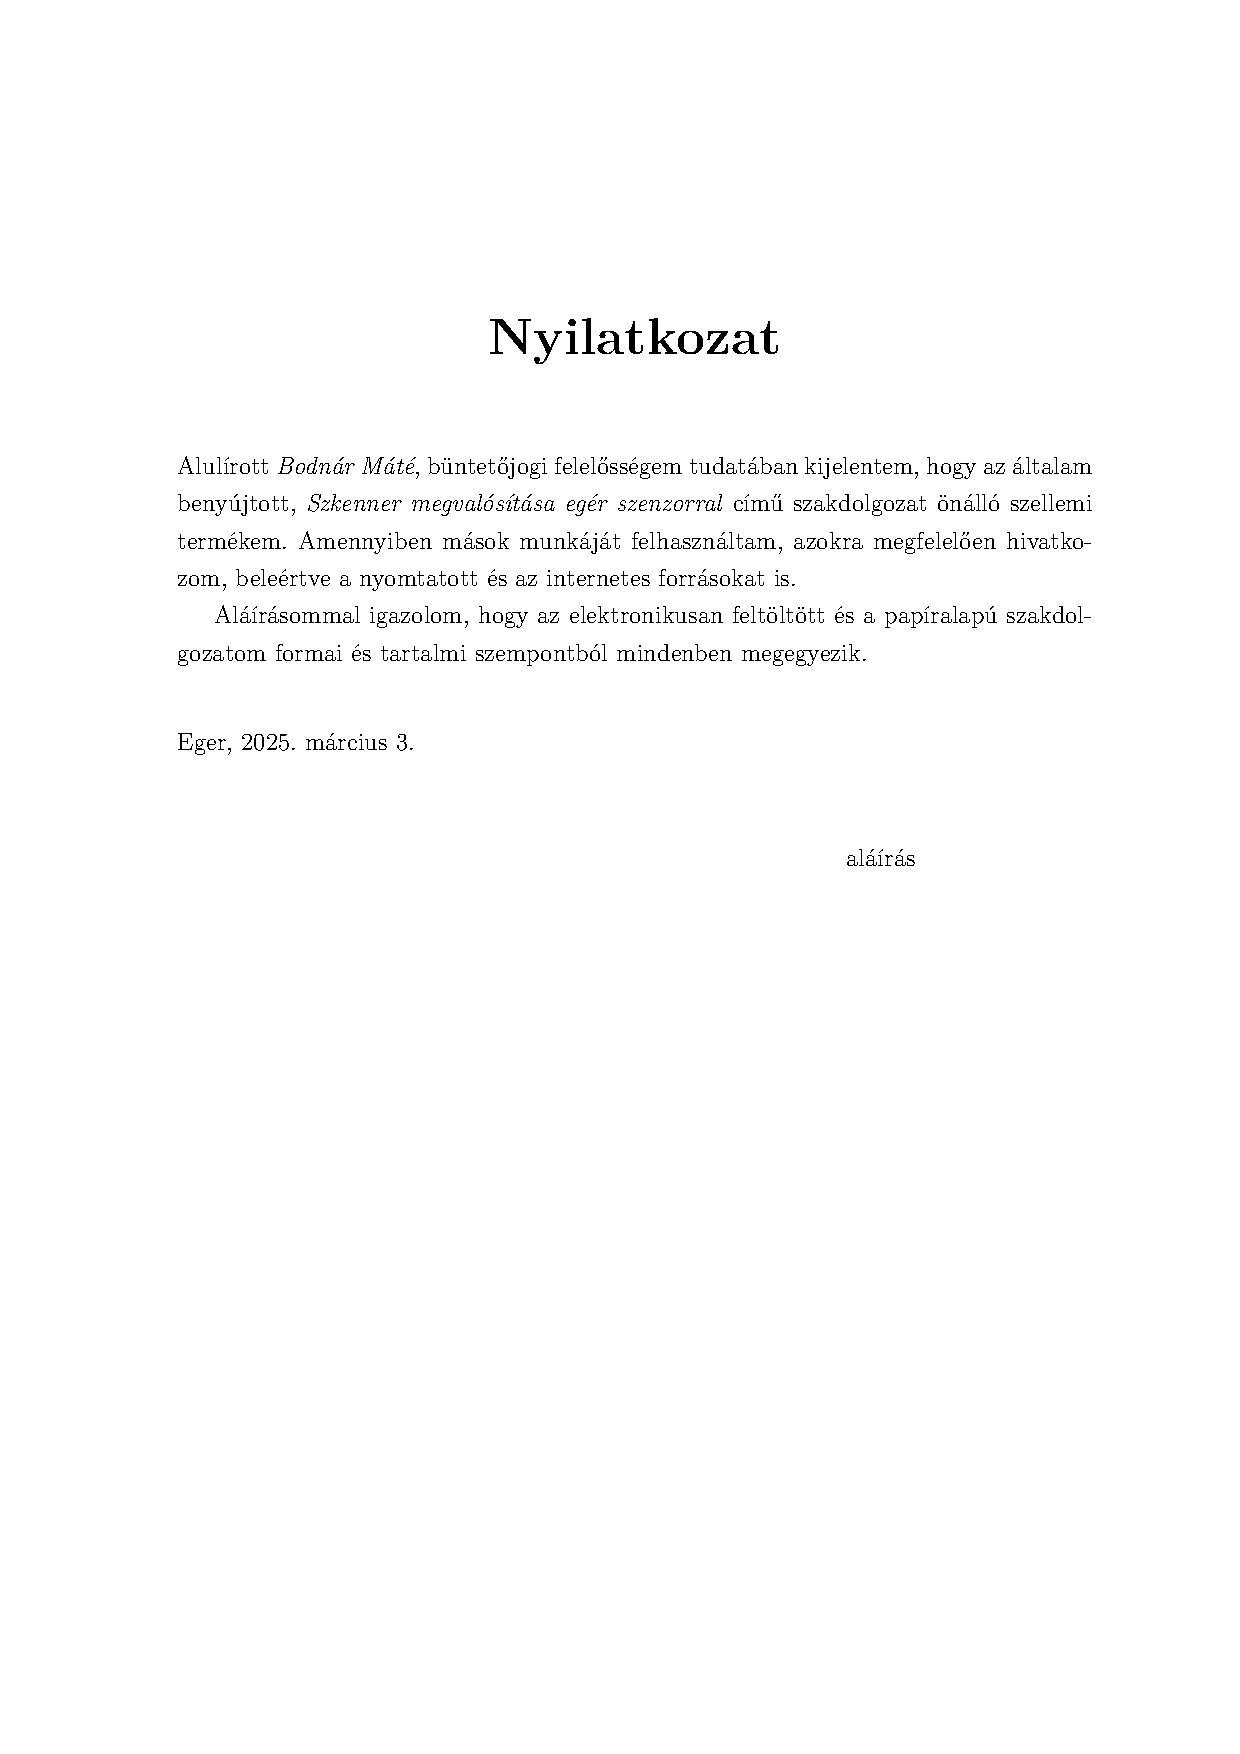
\includepdf{nyilatkozat.pdf}

\end{document}
